% Chang Liu's practice for lshort chapter 3

\documentclass{article}
\usepackage{amssymb}
\usepackage{graphicx}
\usepackage{amsmath} % for bold font
\author{Chang Liu}
\title{Math in \LaTeX{}}

\begin{document}
\maketitle

\newpage


\section{AAA}

Add $a$ squared and $b$ squared
to get $c$ squared. Or, using
a more mathematical approach:
$c^{2}=a^{2}+b^{2}$


\TeX{} is pronounced as
$\tau\epsilon\chi$.\\[6pt]
100~m$^{3}$ of water\\[6pt]
This comes from my $\heartsuit$

Add $a$ squared and $b$ squared
to get $c$ squared. Or, using
a more mathematical approach:
\begin{displaymath}
c^{2}=a^{2}+b^{2}
\end{displaymath}
And just one more line.

\begin{equation} \label{eq:eps} % here we name a new lable and in the next part we give a new reference to it
\epsilon > 0
\end{equation}

From (\ref{eq:eps}), we gather \ldots % here use \ldots instead of .... % here use a reference, note the () is just for quote


$\lim_{n \to \infty}
\sum_{k=1}^n \frac{1}{k^2}
= \frac{\pi^2}{6}$


$\lim_{n \to \infty}\sum_{k=1}^n \frac{1}{k^2} = \frac{\pi^2}{6}$ %%% NOTE for this equation

\begin{displaymath}
\lim_{n \to \infty}
\sum_{k=1}^n \frac{1}{k^2}
= \frac{\pi^2}{6}
\end{displaymath}


% \forall means everyone, \in means included by..., \mathbf means that bold in math equation.
\begin{equation}
\forall x \in \mathbf{R} % between the lines should no blank line
\qquad x^2 \geq 0 % >= means \geq  meaning
\end{equation}

\begin{equation}
x^{2} \geq 0\qquad
\textrm{for all }x\in\mathbf{R}
\end{equation}

\begin{displaymath}
x^{2} \geq 0\qquad
\textrm{for all }x\in\mathbb{R}
\end{displaymath}


\begin{equation}
a^x+y \neq a^{x+y}
\end{equation}


\section{BBB: special math character and its model}

$\lambda,\xi,\pi,\mu,\Phi,\Omega$

$\alpha, \beta, \gamma$

$\Delta, \Gamma$

$a_{1}$ \qquad $x^{2}$ \qquad
$e^{-\alpha t}$ \qquad
$a^{3}_{ij}$\\
$e^{x^2} \neq {e^x}^2$

$\sqrt{x}$ \qquad
$\sqrt{ x^{2}+\sqrt{y} }$
\qquad $\sqrt[3]{2}$\\[3pt]
$\surd[x^2 + y^2]$

$\overline{m+n}$ \qquad
$\underline{m+n}$

$\underbrace{ a+b+\cdots+z }_{26}$

\begin{displaymath}
\vec a\quad\overrightarrow{AB}
\end{displaymath}

\begin{displaymath}
v = {\sigma}_1 \cdot {\sigma}_2
{\tau}_1 \cdot {\tau}_2
\end{displaymath}

%%%%%%%%%%%%%%%%%%%%%%%%%%%%%%%%%%%%%%%%%%%%%%%%%%%%%%%%%%%%%%%%%%%%%%%%5
%\arccos \cos
%\csc \exp
%\ker
%\limsup \min
%\arcsin \cosh \deg \gcd \lg \ln \Pr
%\arctan \cot \det \hom \lim \log \sec
%\arg \coth \dim \inf \liminf \max \sin
%\sinh \sup \tan \tanh
%%%%%%%%%%%%%%%%%%%%%%%%%%%%%%%%%%%%%%%%%%%%%%%%%%%%%%%%%%%%%%%%%%%%%%%%
\[\lim_{x \rightarrow 0}
\frac{\sin x}{x}=1\] % \[ === $


$\lim_{x \rightarrow 0} 
\frac{\sin x}{x}=1$  % \[ is equal to the begin{displaymath}, which gives a better result of math display

\begin{displaymath}
{n \choose k}\qquad {x \atop y+2}
\end{displaymath}

\begin{displaymath}
\int f_N(x) \stackrel{!}{=} 1
\end{displaymath}

%% jifen operation is by \int
%% qiuhe operation is by \sum
%% chengji operation is by \prod

\begin{displaymath}
\sum_{i=1}^{n} \qquad
\int_{0}^{\frac{\pi}{2}} \qquad
\prod_\epsilon
\end{displaymath}

$\Big( (x+1) (x-1) \Big) ^{2}$\\
$\big(\Big(\bigg(\Bigg($\quad
$\big\}\Big\}\bigg\}\Bigg\}$\quad
$\big\|\Big\|\bigg\|\Bigg\|$


\section{CCC: blank in math equation}

\newcommand{\ud}{\mathrm{d}}
\begin{displaymath}
\int\!\!\!\int_{D} g(x,y)
\, \ud x\, \ud y
\end{displaymath}
instead of
\begin{displaymath}
\int\int_{D} g(x,y)\ud x \ud y
\end{displaymath}


\begin{center}
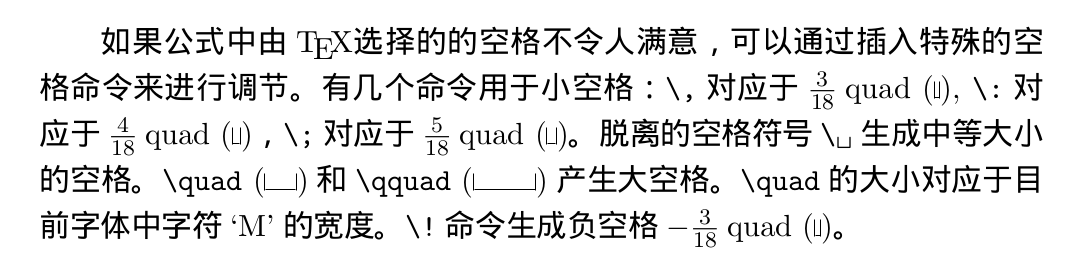
\includegraphics[scale=0.25]{lshort_ch3.png}
\end{center}

\begin{displaymath}
\mathbf{X} =
\left( \begin{array}{ccc}
x_{11} & x_{12} & \ldots \\
x_{21} & x_{22} & \ldots \\
\vdots & \vdots & \ddots
\end{array} \right)
\end{displaymath}


\begin{displaymath}
y = \left\{ \begin{array}{ll}
a & \textrm{if $d>c$}\\
b+x & \textrm{in the morning}\\
l & \textrm{all day long}
\end{array} \right.
\end{displaymath}


\begin{displaymath}
\left(\begin{array}{c|c}
1 & 2 \\
\hline
3 & 4
\end{array}\right)
\end{displaymath}

\begin{eqnarray}
f(x) & = & \cos x
\\
f’(x) & = & -\sin x
\\
\int_{0}^{x} f(y)dy &
= & \sin x
\end{eqnarray}

{\setlength\arraycolsep{2pt}
\begin{eqnarray}
\sin x & = & x -\frac{x^{3}}{3!}
+\frac{x^{5}}{5!}-{}
\nonumber\\
& & {}-\frac{x^{7}}{7!}+{}\cdots
\end{eqnarray}}

\begin{eqnarray}
\lefteqn{ \cos x = 1
-\frac{x^{2}}{2!} +{} }
\nonumber\\
& & {}+\frac{x^{4}}{4!}
-\frac{x^{6}}{6!}+{}\cdots
\end{eqnarray}

\begin{displaymath}
{}^{12}_{\phantom{1}6}\textrm{C}
\qquad \textrm{versus} \qquad
{}^{12}_{6}\textrm{C}
\end{displaymath}


\begin{displaymath}
\Gamma_{ij}^{\phantom{ij}k}
\qquad \textrm{versus} \qquad
\Gamma_{ij}^{k}
\end{displaymath}

\begin{displaymath}
\mathop{\mathrm{corr}}(X,Y)=
\frac{\displaystyle
\sum_{i=1}^n(x_i-\overline x)
(y_i-\overline y)}
{\displaystyle\biggl[
\sum_{i=1}^n(x_i-\overline x)^2
\sum_{i=1}^n(y_i-\overline y)^2
\biggr]^{1/2}}
\end{displaymath}


\section{DDD: theorm law...}

% definitions for the document
% preamble
\newtheorem{law}{Law}
\newtheorem{jury}[law]{Jury}
%in the document
\begin{law} \label{law:box}
Don’t hide in the witness box
\end{law}
\begin{jury}[The Twelve]
It could be you! So beware and
see law~\ref{law:box}\end{jury}
\begin{law}No, No, No\end{law}


\flushleft
\newtheorem{mur}{Murphy}[section]
\begin{mur}
If there are two or more
ways to do something, and
one of those ways can result
in a catastrophe, then
someone will do it.\end{mur}


\section{EEE: bold}

\begin{displaymath}
\mu, M \qquad \mathbf{M} \qquad
\mbox{\boldmath $\mu, M$}
\end{displaymath}


\begin{displaymath}
\mu, M \qquad
\boldsymbol{\mu}, \boldsymbol{M}
\end{displaymath}


\end{document}


